\documentclass[11pt,letterpaper]{article}

%\usepackage{times}
%\usepackage{epsfig}
\usepackage{graphicx}
%\usepackage{amsmath}
%\usepackage{amssymb}
\usepackage{hyperref}
\usepackage{tabularx}
\usepackage[left=1in, right=1in, top=1in, bottom=1in]{geometry}
\usepackage{titling}
\usepackage{setspace}
\usepackage{sectsty}
\usepackage{tabto}
\graphicspath{{./final_project_phase_1/}} % adds the assets directory to the path, throw your images there
\usepackage{fancyhdr}
\pagestyle{fancy}
\fancyhf{}
\fancyheadoffset{0cm}
\renewcommand{\headrulewidth}{0pt} 
\renewcommand{\footrulewidth}{0pt}
\fancyhead[R]{\thepage}
\fancypagestyle{plain}{%
  \fancyhf{}%
  \fancyhead[R]{\thepage}%
}

\usepackage{cite}
\usepackage[sectionbib]{natbib}
\renewcommand{\refname}{}

\usepackage{rotating}

\begin{document}
\fontfamily{ptm}\selectfont
\sectionfont{\fontsize{12}{12}\fontfamily{ptm}\selectfont}
\doublespacing
%%%%%%%%%%%%%%%%%%%%%%%%%%%%%% TITLE %%%%%%%%%%%%%%%%%%%%%%%%%%%%%%%%%%%%%%
\setlength{\droptitle}{1in} 

\title{\large{AI AGENT-POWERED AUTOMATION FOR PELOTON FITNESS ECOSYSTEM: \\ REQUIREMENTS ANALYSIS PHASE \\\vspace{1.2in}}}

\author{
Kevin Geidel \\
MSDS 442: AI Agent Design \& Development \\
Northwestern University \\
May 4, 2025 \\
}

\date{}
\maketitle
\thispagestyle{empty}	
\clearpage
\setcounter{page}{1}

%%%%%%%%%%%%%%%%%%%%%%%%%%%%%% PAGE 1 %%%%%%%%%%%%%%%%%%%%%%%%%%%%%%%%%%%%
\section*{Requirements analysis overview}
\tab The goal of the Peloton project is to design and implement a suite of multimodal AI agents that provide automation in a few key areas of the Peloton ecosystem (Order/Shipping, Product Management, Marketing, Membership \& Fraud Detection and Data Science.)
These agents must leverage \textit{Large Language Models (LLMs)} and other AI modalities (image/document processing, querying structured data, etc) to handle tasks such as order tracking, product cataloging, marketing campaign performance analysis, fraud detection, user/customer segmentation, and predictive analytics. 
The aim is to create an intelligent, AI-driven tool that improves operational efficiency, customer engagement, decision-making and scalability for Peloton.

The ChatGPT (\url{chatgpt.com}) conversational client was used to analyze the project requirements (see figure \ref{fig:load_reqs}). 
Its responses have been evaluated along side my own and combined to make a clear picture of how the Peloton project should be approached and how to support decision making in regards to implementation.

\section*{Requirement 1: Feasibility of a multimodal LLM-based agent}
\tab There are many opportunities for automation using LLM based AI agents in the Peloton project requirements.
When requirement \#1 was analyzed by ChatGPT (figure \ref{fig:req1}) the chat bot pointed out some important caveats to this.
However, on the whole, it will be possible to meet the project requirements using multimodal AI agents. By divvying up process and workflows into
different `nodes' and `edges' on an AI agent graph we can have each agent node focus on a specific portion of the desired capabilities.
The complete Peloton project will be the sum of each agent working in concert.

The ChatGPT response did mention that full automation will require `deterministic' components. I think this is a great point but does not prevent us from achieving automation. For example, it is true that an LLM is not appropriate for processing secure payments. We can address this by providing the respective agent responsible for membership support the payment portal as an external tool. If the agent determines the user is trying to make a payment they can be forwarded to the payment portal where our conventional server-side application can be used to complete the transaction.
This could look like what we did in virtual lab \#2, providing our own functions as external actions to the agent. In this example, the member support agent would utilize a \texttt{forward\_to\_payment\_portal} action once it determined that was what the user required.

\section*{Requirement 2: Considering user stories}
\tab Developing user-stories is a common project management exercise that helps keep the end goal of the project in the forefront of design.
User-stories should be specific, realistic and implementable. If we create stories that span all project requirements and our final product can perform in each of these scenarios we know the desired capabilities have been delivered. ChatGPT was prompted for three user-stories for each of the five key business areas (that correspond to the five main agents in the envisioned architecture.) Figure \ref{fig:req2} shows the exchange with ChatGPT and its output.

These 15 user-stories make a great starting point for target capabilities. During development these will be used like a checklist, making sure the tool can accomplish these tasks and handle related prompts properly. This list also gives us cues about the types of external tools that we will need to make available for the agents. For example, there is a user-story involving the marketing agent providing recent social media trends. In order to accommodate this story the agent will need access to a general web search to get the latest trends. In virtual lab \#3 we made Tavily available to the agent for getting current weather reports. We can use this same technique to make recent trends available to the agent in support of this user-story (and others!)

\section*{Requirement 3: Design with user stories in mind}
\tab When requirement \#3 was provided to ChatGPT (see figure \ref{fig:req3}) the output was a series of well formatted Markdown tables that provided a summary of the design and implementation approach for each of the 15 user-stories. These summaries are reproduced in table \ref{table:stories} for easier viewing.

By examining the implementation notes in detail we have more insight into the techniques required to deliver the required capability. Consider the user stories for the product recommendations agent. Each of these stories involve access to structured data, namely sales and user activity records. In virtual lab \#4 we loaded a variety of documents (including some with structured data) into the prompt context using \textit{Retrieval Augmented Generation (RAG)} techniques. This involved creating embeddings of open text fields, placing them in a vector store and creating retrieval tools for the agent to utilize as needed.
This design approach can be used in support of these user-stories that benefit from access to enterprise data such as sales records.

\section*{Requirement 4: Training \& test data}
\tab The development of these five AI agents (and the agent that will direct user queries to the appropriate agent) will require populated tables of structured data (sales records, product descriptions, user accounts, etc) and example user queries with their expected outputs.
Figure \ref{fig:req4} shows the initial exchange with ChatGPT after seeing requirement \#4. The response lays out the sort of training data that would be needed to test each of the agents. 

This was followed up with specific requests for example data sets that related to each of the five areas. The responses consisted of Markdown tables whose rows correlated to records pertaining to that given business area. For example, ChatGPT generated faux order data that have been reformatted and displayed in table \ref{table:orders}. Similar data sets were obtained for product data, marketing campaign metrics, user/membership access records and user/customer performance metrics as shown in figures \ref{fig:products} through \ref{fig:ds} respectively.
The generated data sets will be a surrogate for the external data sources that a production enterprise system would have. The Peloton AI agents will need access to tables like these and the records produced by ChatGPT are a starting point that will enable development to begin. Upon request, ChatGPT made all of these records available for download in a single \texttt{JSON} file. This file will be chunked up and loaded into the various RAG tools we develop as part of the project.

In addition to having records that simulate populated enterprise systems it would be useful to have a list of hypothetical user prompts that represent each of the user-stories. In figure \ref{fig:prompts} you can see a series of user queries and their expected outputs. These span the five domains governed by each of the AI agents and will provide a great benchmark for measuring progress while developing the project.

\pagebreak
\section*{\center{Appendix}}

\begin{figure}[h]
    \centering
      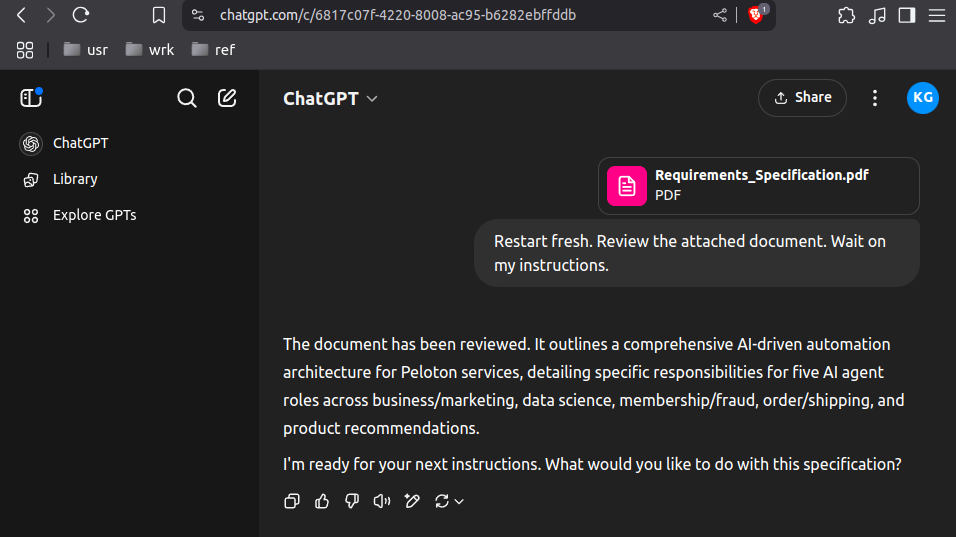
\includegraphics[width=1.0\linewidth]{chatgpt_01.png}
      \caption{Loading project requirements on \url{chatgpt.com}}
    \label{fig:load_reqs}
\end{figure}

\begin{figure}[h!]
    \centering
      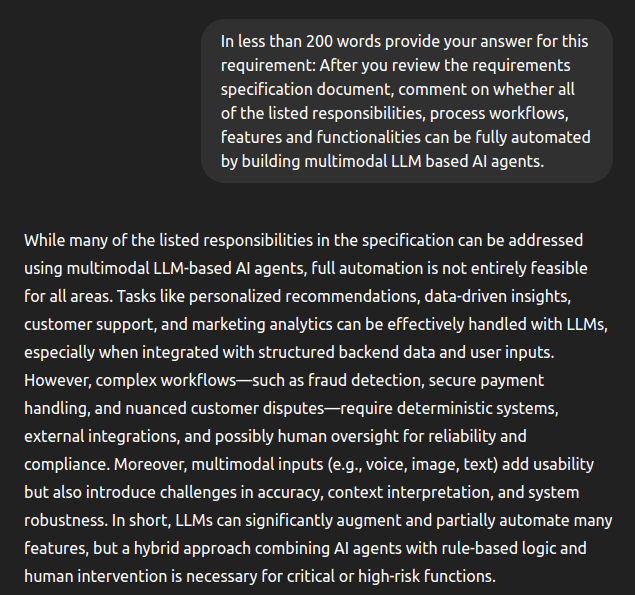
\includegraphics[width=1.0\linewidth]{chatgpt_02.png}
      \caption{ChatGPT analyzed requirement \#1 and notes automation opportunities.}
    \label{fig:req1}
\end{figure}

\begin{figure}[h!]
    \centering
      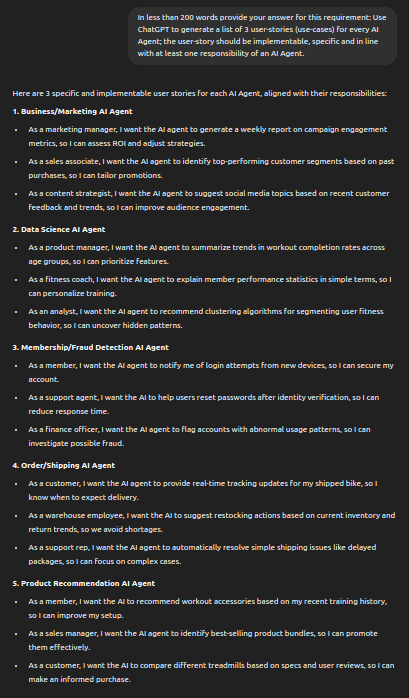
\includegraphics[width=0.75\linewidth]{chatgpt_03.png}
      \caption{ChatGPT wrote user-stories for each key area in requirement \#2.}
    \label{fig:req2}
\end{figure}

\begin{figure}[h!]
    \centering
      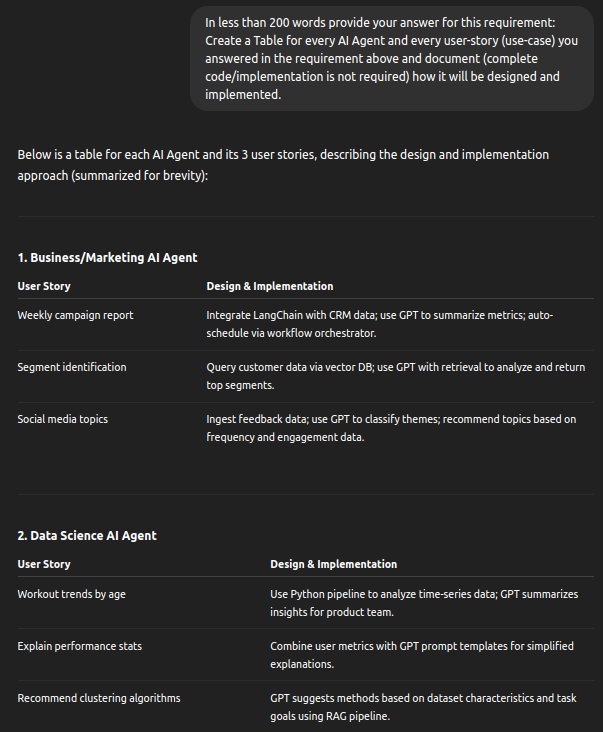
\includegraphics[width=0.5\linewidth]{chatgpt_04a.png}
      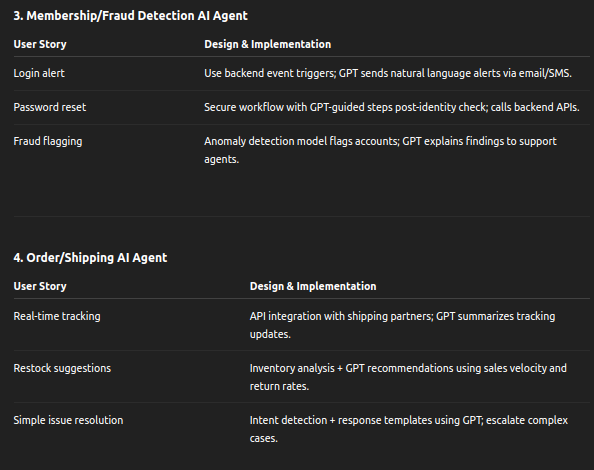
\includegraphics[width=0.5\linewidth]{chatgpt_04b.png}
      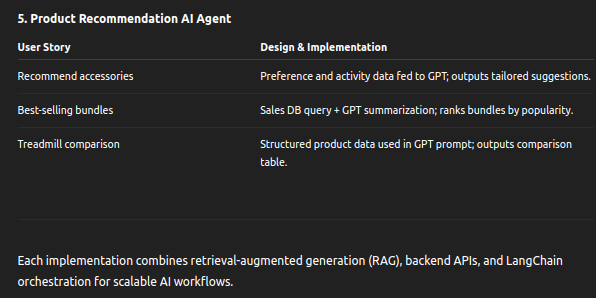
\includegraphics[width=0.5\linewidth]{chatgpt_04c.png}      
      \caption{ChatGPT broke down each user-story for requirement \#3.}
    \label{fig:req3}
\end{figure}

\clearpage

\begin{table}[h!]
    \centering
    \begin{tabular}{l p{.5\linewidth}}
User Story             & Design \& Implementation \\ \hline
\multicolumn{2}{l}{1. Business/Marketing AI Agent} \\
\hline
Weekly campaign report & Integrate LangChain with CRM data; use GPT to summarize metrics; auto-schedule via workflow orchestrator.  \\
Segment identification & Query customer data via vector DB; use GPT with retrieval to analyze and return top segments.              \\
Social media topics    & Ingest feedback data; use GPT to classify themes; recommend topics based on frequency and engagement data. \\
\hline        
\multicolumn{2}{l}{2. Data Science AI Agent} \\
\hline
Workout trends by age           & Use Python pipeline to analyze time-series data; GPT summarizes insights for product team. \\
Explain performance stats       & Combine user metrics with GPT prompt templates for simplified explanations.                \\
Recommend clustering algorithms & GPT suggests methods based on dataset characteristics and task goals using RAG pipeline.   \\
\hline
\multicolumn{2}{l}{3. Membership/Fraud Detection AI Agent} \\
\hline
Login alert    & Use backend event triggers; GPT sends natural language alerts via email/SMS.     \\
Password reset & Secure workflow with GPT-guided steps post-identity check; calls backend APIs.   \\
Fraud flagging & Anomaly detection model flags accounts; GPT explains findings to support agents. \\
\hline
\multicolumn{2}{l}{4. Order/Shipping AI Agent} \\
\hline
Real-time tracking      & API integration with shipping partners; GPT summarizes tracking updates. \\
Restock suggestions     & Inventory analysis + GPT recommendations using sales velocity and return rates. \\
Simple issue resolution & Intent detection + response templates using GPT; escalate complex cases. \\
\hline
\multicolumn{2}{l}{5. Product Recommendation AI Agent} \\
\hline
Recommend accessories & Preference and activity data fed to GPT; outputs tailored suggestions. \\
Best-selling bundles  & Sales DB query + GPT summarization; ranks bundles by popularity.       \\
Treadmill comparison  & Structured product data used in GPT prompt; outputs comparison table.  \\
    \end{tabular}
    \caption{ChatGPT's user-stories broken down.}
    \label{table:stories}
  \end{table}

\clearpage

\begin{figure}[h!]
    \centering
      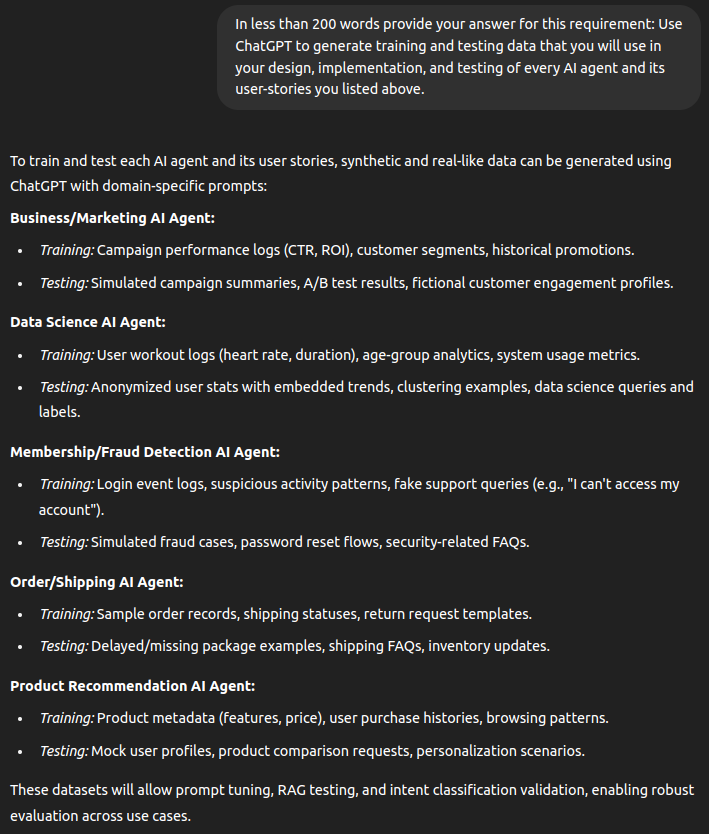
\includegraphics[width=1.0\linewidth]{chatgpt_05.png}    
      \caption{ChatGPT, prompted with requirement \#4, gave advice on obtaining test data.}
    \label{fig:req4}
\end{figure}

\clearpage

\begin{sidewaystable}[h!]
    \centering
    \begin{tabular}{p{1.1cm} p{1.8cm} p{1.8cm} p{1.8cm} p{1.8cm} p{1.8cm} p{1.8cm} p{1.8cm} p{1.5cm} p{1.8cm}}
Order ID & Customer Name & Product & Order Date & Shipping Status & Delivery Date & Carrier & Tracking Number & Issue Reported  & Resolution Status   \\
\hline
ORD001 & Sarah Collins     & Peloton Bike+        & 2025-04-10 & Shipped & 2025-04-15   & FedEx & FX123... & None & N/A \\
ORD002 & James Patel       & Tread                & 2025-04-12 & Delayed & 2025-04-20   & UPS   & 1Z999... & Weather delay & Pending     \\
ORD003 & Maria Gonzalez    & Bike Mat + Shoes     & 2025-04-13 & Delivered & 2025-04-17 & USPS  & 94001... & None & N/A \\
ORD004 & Kevin Wu          & Dumbbell Set         & 2025-04-14 & In Transit & 2025-04-19 & DHL  & DHL98... & None & N/A \\
ORD005 & Linda Harper      & Heart Rate Monitor   & 2025-04-10 & Delivered & 2025-04-13 & FedEx & FX876... & Missing item & Under Investigation     \\
ORD006 & Omar Siddiqui     & Apparel Bundle       & 2025-04-11 & Returned & 2025-04-16  & UPS   & 1Z888... & Size issue & Refunded    \\
ORD007 & Aisha Khan        & Resistance Bands     & 2025-04-13 & Out for Delivery & 2025-04-18   & USPS        & 94001... & None    & N/A         \\
ORD008 & Daniel Cho        & Peloton Guide        & 2025-04-09 & Lost in Transit & N/A & FedEx & FX000... & Not received & Replacement Shipped \\
ORD009 & Rachel Adams      & Yoga Accessories Set & 2025-04-15 & Processing & 2025-04-22   & N/A & N/A & None    & N/A \\
ORD010 & Marcus Lee        & Water Bottle         & 2025-04-12 & Delivered & 2025-04-14   & USPS & 94001... & Wrong item received & Replacement In Progress \\
        
    \end{tabular}
    \caption{ChatGPT's generated order data (tracking numbers truncated for readability).}
    \label{table:orders}
  \end{sidewaystable}

\clearpage

  \begin{figure}[h!]
    \centering
      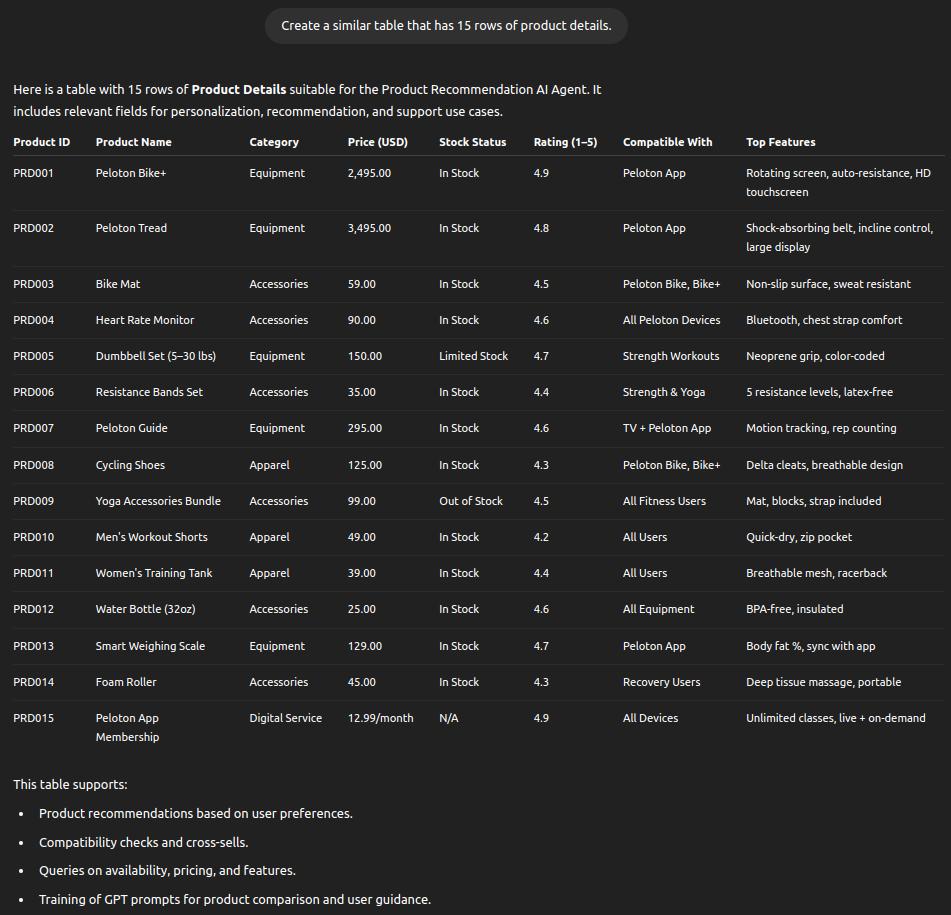
\includegraphics[width=1.0\linewidth]{chatgpt_07.png}    
      \caption{ChatGPT's generated product data.}
    \label{fig:products}
\end{figure}

\begin{figure}[h!]
    \centering
      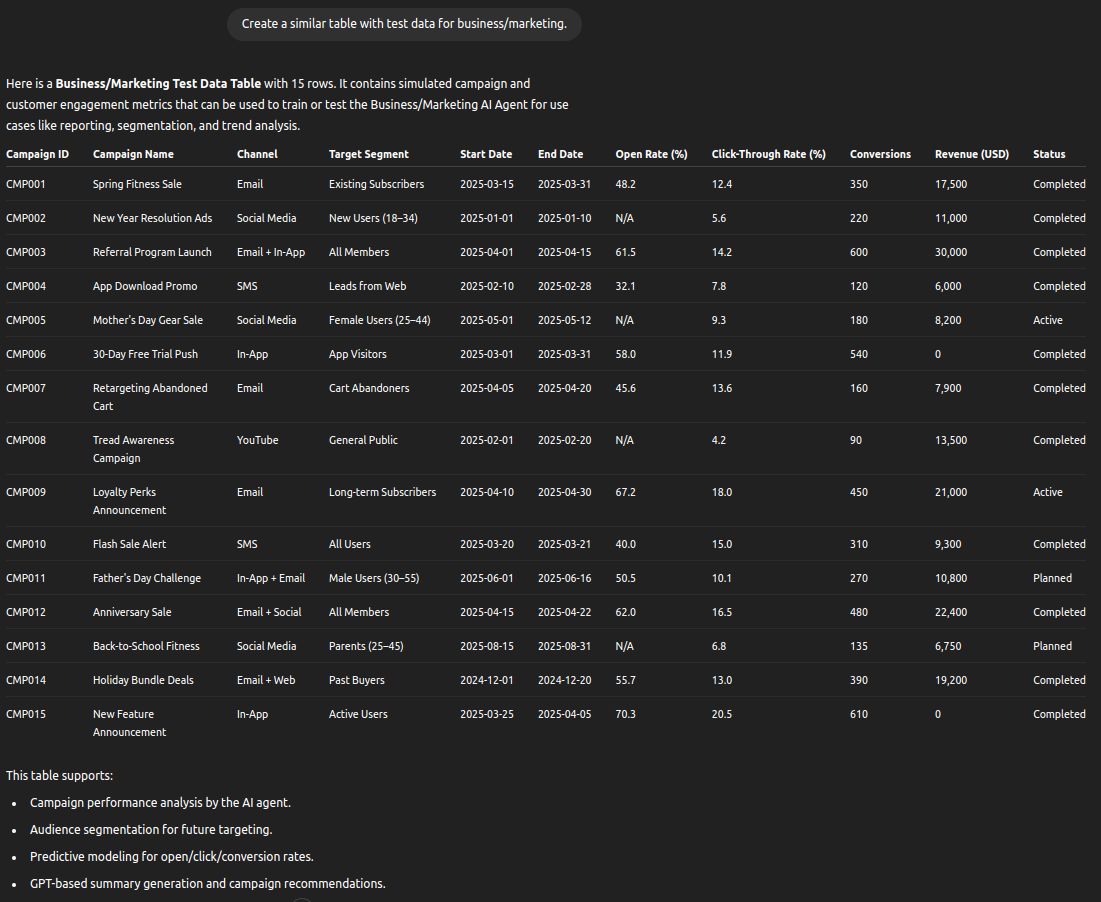
\includegraphics[width=1.0\linewidth]{chatgpt_08.png}    
      \caption{ChatGPT's generated marketing campaign data.}
    \label{fig:marketing}
\end{figure}

\begin{figure}[h!]
    \centering
      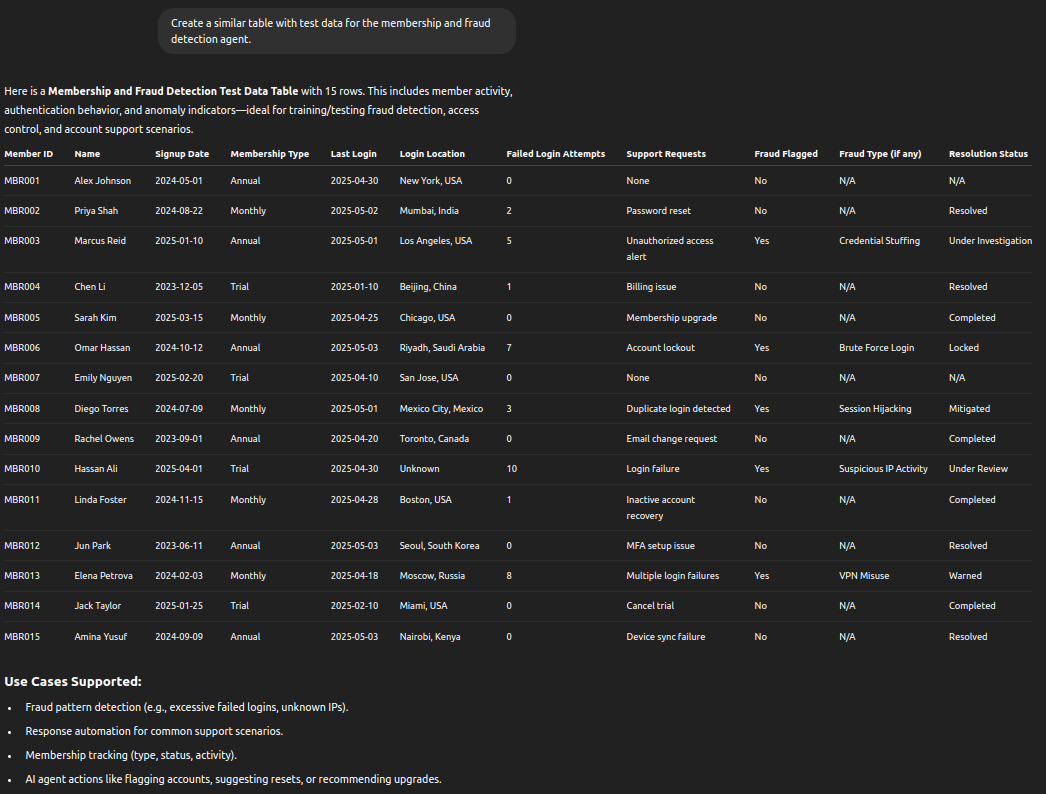
\includegraphics[width=1.0\linewidth]{chatgpt_09.png}    
      \caption{ChatGPT's generated membership and fraud data.}
    \label{fig:membership}
\end{figure}

\begin{figure}[h!]
    \centering
      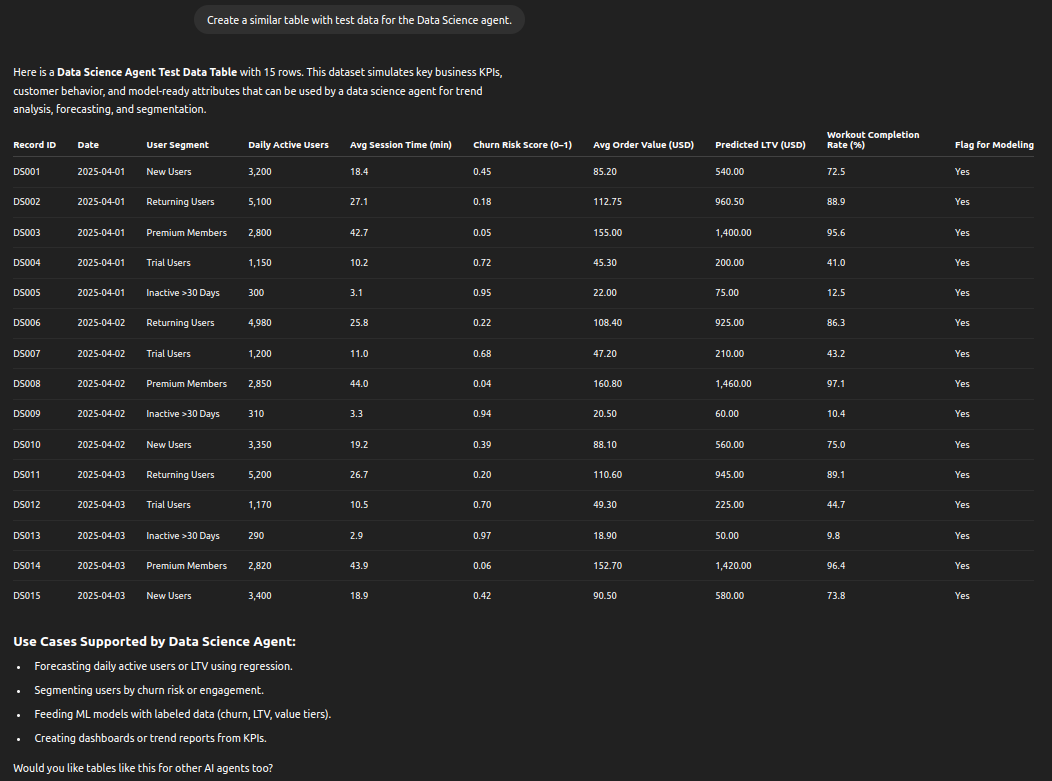
\includegraphics[width=1.0\linewidth]{chatgpt_10.png}    
      \caption{ChatGPT's generated data science and analytics data.}
    \label{fig:ds}
\end{figure}

\begin{figure}[h!]
    \centering
      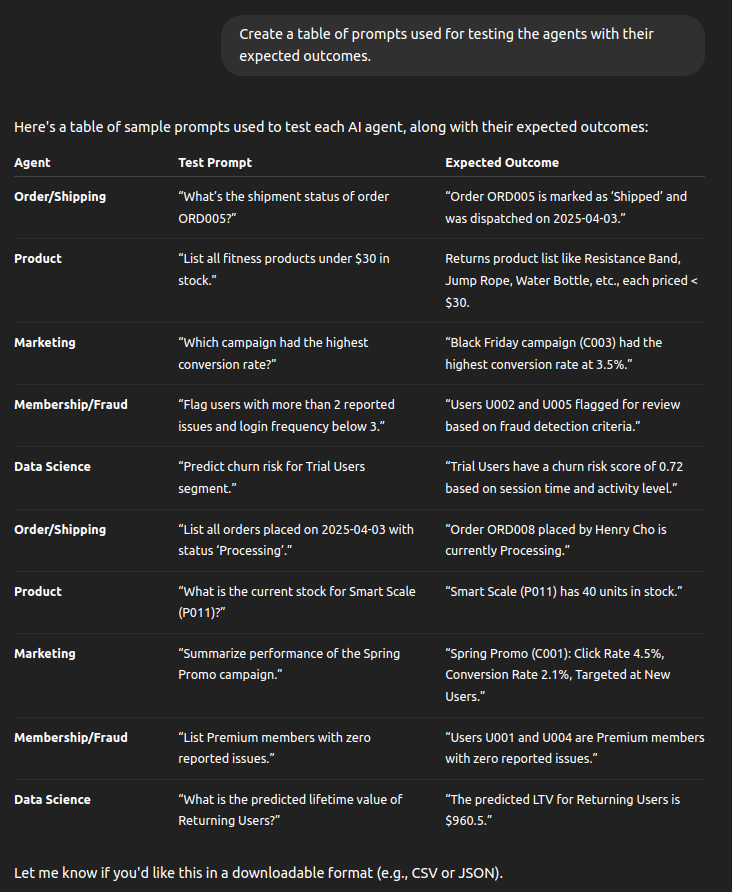
\includegraphics[width=1.0\linewidth]{chatgpt_11.png}    
      \caption{ChatGPT's generated list of hypothetical user queries and expected output.}
    \label{fig:prompts}
\end{figure}

\end{document}